\documentclass[14pt]{memoir}
\setulmarginsandblock{2cm}{2cm}{*}
\setlrmarginsandblock{1.5cm}{1.5cm}{*}
\checkandfixthelayout
\usepackage[spanish,activeacute,es-tabla]{babel}
\usepackage{amsmath}
\usepackage{amssymb,latexsym}
\usepackage[spanish]{layout}
\usepackage{graphicx} 
\usepackage{bigints}
\usepackage{hyperref} 
\usepackage[utf8]{inputenc}

\begin{document}

\begin{center}
			\centering
			Actividad No. $(2)$\\
			$2024$ Cálculo Vectorial.\\
			Nombres:  Camilo Rivera, Emerson Tavera, Karen Torres
\end{center}

\begin{enumerate}

	\item[ 1] Diga si la afirmación es verdadera o falsa. Justifique sus respuestas: 
	
	
	
	\item[ a)] La gráfica del dominio de $f(x, y) = \ln(9x^2 - y^2 - 9)$ \\
	\begin{center}
	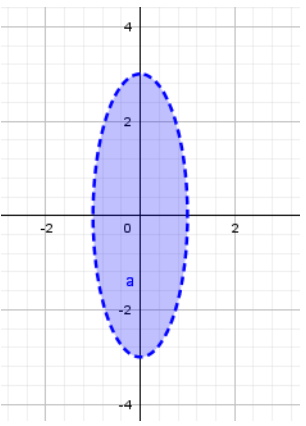
\includegraphics[scale=1]{assets/t_2_1.png} 
	\end{center}
	
	R// Falso\\
	\text{Pues Dada la función: } $f(x, y) = \ln(9x^2 - y^2 - 9)$ \\
	$9x^2 - y^2 - 9 > 0$\\
	$9x^2 - y^2 > 9$\\
	$x^2 - \frac{y^2}{9} > 1$\\ 
	
	lo que representado gráficamente es:
	\begin{center}
	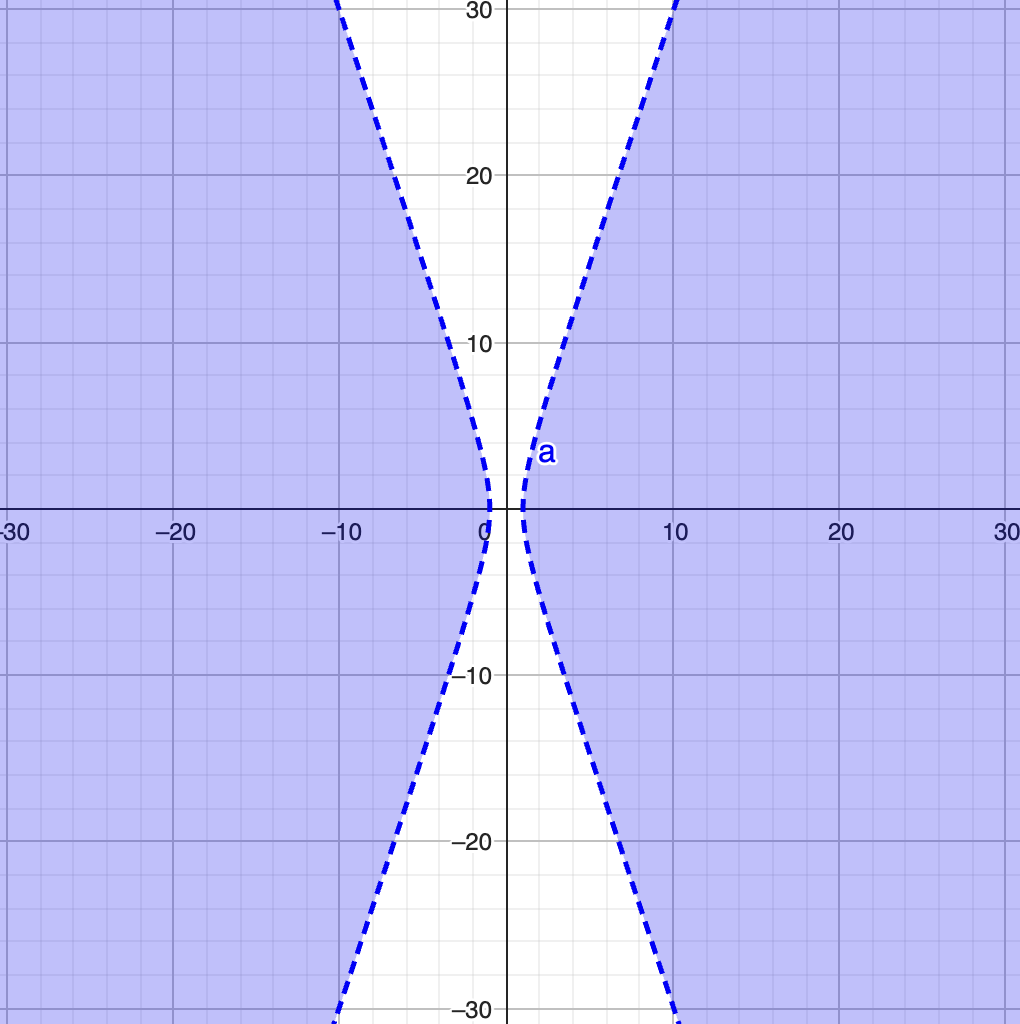
\includegraphics[scale=0.3]{assets/t_2_2.png} 
	\end{center}
	
	
\item[ b)] $F_{xx} = \frac{1}{2\cos(x)}; \;Si\;  f(x, y) = \int_y^x \ln(\cos(t)) \, dt.$ \\
	
$f(x, y) = \int_y^x \ln(\cos(t)) \, dt $ \\

{\tiny \(f_x\) teorema fundamental del cálculo}\\
$f_x = \frac{\partial}{\partial x} \int_y^x \ln(\cos(t)) \, dt = \ln(\cos(x))$\\

{\tiny\(f_{xx}\)  regla de la cadena para diferenciar \(f_x\) con respecto a \(x\):}\\
$f_{xx} = \frac{d}{dx} \ln(\cos(x)) = \frac{1}{\cos(x)} \cdot (-\sin(x)) = -\tan(x)$\\

\textbf{ R// Falso} $f_{xx} = -\tan(x) \neq \frac{1}{2\cos(x)}$\\

\item[ c)] $F_{yy} = \frac{y}{\cos(y)}; \; Si \;f(x, y) = \frac{\sin(x+y)}{x} $ \\

$f(x, y) = \frac{\sin(x+y)}{x}$\\

	
	
\end{enumerate}	

\end{document}